\documentclass[10pt,twocolumn]{article}
\usepackage[utf8]{inputenc}
\usepackage[T1]{fontenc}
\usepackage{amsmath,amssymb,graphicx,booktabs,geometry,hyperref,tikz}
\usetikzlibrary{shapes,arrows.meta,positioning}
\geometry{a4paper,margin=1.6cm,columnsep=0.6cm}
\setlength{\parskip}{2pt}
\title{\vspace{-1.2cm}Predicci\'on Lineal Subbanda: \\ ¿Mejora el procesamiento multitasa la compresi\'on LPC?}
\author{Noel Antonio Perez Caceres}
\date{}
\renewcommand{\figurename}{Fig.}\renewcommand{\tablename}{Tabla}\renewcommand{\abstractname}{Resumen}\renewcommand{\refname}{Referencias}
\begin{document}
\maketitle
\begin{abstract}
Se implementa un codificador LPC-10 y una variante que aplica LPC a cada banda de una descomposici\'on QMF en \'arbol. Se barren 100 configuraciones (niveles, \'ordenes por banda y ventanas) sobre dos audios de referencia (8 y 16~kHz) con distancia log-espectral, y se eval\'uan las configuraciones representativas con PEAQ (ITU-R BS.1387). La descomposici\'on subbanda \emph{no} logr\'o mayor compresi\'on que el LPC tradicional con ventana ajustada para una calidad perceptual equivalente. Se discuten las causas y limitaciones.
\end{abstract}

\section{Introducci\'on y estado del arte}
LPC modela la envolvente espectral con un filtro todo-polos y transmite coeficientes, ganancia, tono y sonoridad en lugar de muestras~\cite{atal71,tremain82}. Funciona bien en voz, pero un modelo todo-polos de orden bajo representa mal espectros de banda ancha como el de la m\'usica. Las l\'ineas de mejora m\'as conocidas son la excitaci\'on por c\'odigo (CELP)~\cite{schroeder85}, que reemplaza el modelo impulsos/ruido por una excitaci\'on optimizada, y la codificaci\'on por subbandas~\cite{crochiere76}, que divide la se\~nal en bandas para asignar bits seg\'un su importancia perceptual. Los bancos de espejo en cuadratura (QMF)~\cite{esteban77,johnston80,vaid93} permiten esa divisi\'on con diezmado y reconstrucci\'on casi perfecta. Este trabajo combina ambas ideas de forma m\'inima: LPC b\'asico aplicado a cada subbanda. La calidad perceptual objetiva se mide con PEAQ (ITU-R BS.1387)~\cite{bs1387}.

\section{Fundamentos}
\textbf{LPC.} Para cada ventana, $\tilde x(n)=\sum_{k=1}^{p}a_k\tilde x(n-k)+G\,e(n)$, con $H(z)=G/(1-\sum_{k=1}^{p}a_kz^{-k})$. Los $a_k$ resuelven las ecuaciones de Yule-Walker $\mathbf R\mathbf a=\mathbf r$ (autocorrelaci\'on, Toeplitz) y $G^2$ es el error de predicci\'on. Es la soluci\'on de Wiener-Hopf para un proceso estacionario en cada ventana (resoluble con Levinson-Durbin), y $|H(e^{j\omega})|^2$ aproxima la densidad espectral de potencia de la ventana. La excitaci\'on es un tren de impulsos de periodo $T$ (voiced) o ruido blanco (unvoiced).

\textbf{Procesamiento multitasa.} Un diezmador por $M$ reduce la tasa a $f_s/M$ y puede producir aliasing si no se filtra antes; un interpolador inserta ceros y requiere filtrado de imagen. En un banco de dos canales, la elecci\'on $G_0(z)=H_0(z)$, $G_1(z)=-H_1(z)$ cancela el aliasing, y la distorsi\'on de amplitud restante depende de $|H_0|^2+|H_1|^2$.

\textbf{QMF.} Se emplea un banco ortogonal (CQF): $h_1[n]=(-1)^n h_0[N-1-n]$ y filtros de s\'intesis invertidos en el tiempo, con $|H_0(\omega)|^2+|H_0(\pi-\omega)|^2=\text{cte}$ para reconstrucci\'on casi perfecta. Un \'arbol de $L$ niveles sobre la rama baja genera $L+1$ bandas de anchos $f_{\max}/2^L,\,f_{\max}/2^L,\dots,f_{\max}/2$.

\textbf{Compresi\'on.} $\mathrm{CR}=16\,n_{\text{muestras}}\,/\,B$, con $B=\sum_{\text{ventanas}}(p\,b_c+b_G+b_v+b_T\,\mathbb 1_{\text{voiced}})$ y $b_c=8$, $b_G=5$, $b_v=1$, $b_T=7$~bits (supuestos).

\section{Soluci\'on propuesta}
\begin{figure}[t]\centering
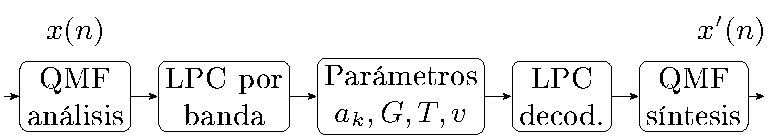
\includegraphics[width=\columnwidth]{diagrama.pdf}
\caption{Diagrama de bloques: codificador (izquierda) y decodificador (derecha).}\label{fig:blk}
\end{figure}

\textbf{LPC tradicional:} ventanas de 22.5~ms sin traslape (Hamming para LP), pre-\'enfasis $1-0.68z^{-1}$, sonoridad por energ\'ia y ZCR (umbrales $E>5\,\%$ de la media, $ZC<0.25$), tono por autocorrelaci\'on (60--400~Hz), potencia con n\'umero entero de periodos y de-\'enfasis en el decodificador. Orden $p=10$.

\textbf{LPC subbanda:} descomposici\'on QMF en \'arbol de $L\in\{2,3,4\}$ niveles (Fig.~5 del enunciado); cada banda se codifica con el mismo LPC a su frecuencia de muestreo, con orden $p_i$ y ventana propios. El decodificador sintetiza cada banda y recompone con el \'arbol de s\'intesis (Fig.~\ref{fig:blk}) (con compensaci\'on de retardo entre ramas). El filtro de 64 coeficientes reconstruye con error relativo de 2\,\% (\mbox{$\approx-34$~dB}). La Fig.~\ref{fig:qmf} muestra su respuesta en frecuencia.

\begin{figure}[t]\centering
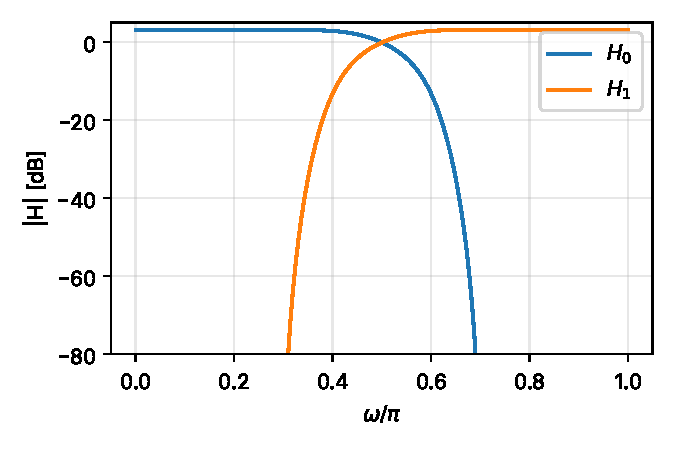
\includegraphics[width=0.8\columnwidth]{qmf_resp.pdf}
\caption{Respuesta en frecuencia de $H_0$ y $H_1$.}\label{fig:qmf}
\end{figure}

\section{Resultados}
\textbf{Metodolog\'ia.} Audios \texttt{referencia\_16k.wav} y \texttt{referencia\_8k.wav} (13.5~s). Se barrieron 50 configuraciones subbanda por audio con la distancia log-espectral (LSD, STFT de 512 puntos; menor es mejor). Las configuraciones representativas, junto con LPC-10 y variantes de ventana del LPC tradicional, se evaluaron con PEAQ (\texttt{peaqb-fast}, ODG) tras remuestrear a 48~kHz y duplicar el canal, como exige la herramienta (Tabla~\ref{tab:cfg}). Las salidas del decodificador se alinean con el original (el retardo del banco, 441 muestras, se compensa).

\begin{figure}[t]\centering
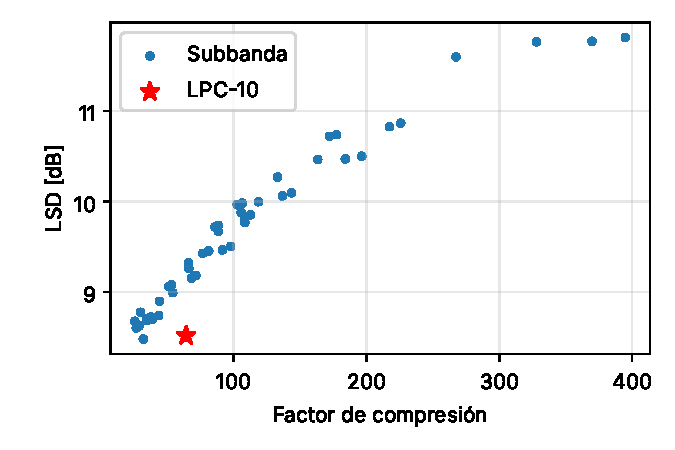
\includegraphics[width=0.85\columnwidth]{cr_vs_lsd_referencia_16k.pdf}
\caption{CR frente a LSD (16~kHz). Cada punto azul es una configuraci\'on subbanda; la estrella es LPC-10.}\label{fig:cr}
\end{figure}

\begin{table*}[t]\centering\footnotesize
\caption{Resultados por audio. Configuraci\'on: \'ordenes $p$ / ventanas [ms] (banda m\'as baja a m\'as alta). ODG: PEAQ (0 imperceptible, $-4$ muy molesto); LSD: distancia log-espectral [dB].}\label{tab:cfg}
\begin{tabular}{lllrrr}\toprule
Audio & Sistema & $p$ / ventana & CR & LSD [dB] & ODG\\\midrule
16~kHz & LPC-10 & 10 / 22.5 & 64.1 & 8.52 & -3.79\\
16~kHz & LPC-10 & 10 / 45 & 128.2 & 9.24 & -3.81\\
16~kHz & LPC-10 & 10 / 90 & 257.0 & 10.31 & -3.84\\
16~kHz & Sub. $L{=}$3 & 12,6,4,2 / 22.5,22.5,22.5,22.5 & 26.6 & 8.6 & -3.86\\
16~kHz & Sub. $L{=}$3 & 10,6,4,2 / 22.5,22.5,22.5,22.5 & 28.8 & 8.63 & -3.86\\
16~kHz & Sub. $L{=}$3 & 10,6,4,2 / 90,45,22.5,22.5 & 53.1 & 9.08 & -3.9\\
16~kHz & Sub. $L{=}$3 & 10,4,2,2 / 90,45,22.5,22.5 & 68.2 & 9.15 & -3.9\\
16~kHz & Sub. $L{=}$2 & 8,4,2 / 360,180,90 & 394.9 & 11.81 & -3.91\\
\midrule
8~kHz & LPC-10 & 10 / 22.5 & 32.3 & 9.18 & -3.61\\
8~kHz & LPC-10 & 10 / 45 & 64.5 & 9.97 & -3.84\\
8~kHz & LPC-10 & 10 / 90 & 129.5 & 12.48 & -3.86\\
8~kHz & Sub. $L{=}$3 & 12,6,4,2 / 22.5,22.5,22.5,22.5 & 13.1 & 9.91 & -3.78\\
8~kHz & Sub. $L{=}$3 & 10,6,4,2 / 22.5,22.5,22.5,22.5 & 14.2 & 9.93 & -3.76\\
8~kHz & Sub. $L{=}$3 & 10,6,4,2 / 90,45,22.5,22.5 & 26.6 & 9.99 & -3.88\\
8~kHz & Sub. $L{=}$3 & 10,4,2,2 / 90,45,22.5,22.5 & 34.1 & 10.18 & -3.88\\
8~kHz & Sub. $L{=}$2 & 8,4,2 / 360,180,90 & 198.4 & 12.74 & -3.91\\
\bottomrule\end{tabular}
\end{table*}

\textbf{Factor de compresi\'on.} LPC-10 (22.5~ms) logra CR $=64.1$ a 16~kHz y $32.3$ a 8~kHz. Las configuraciones subbanda m\'as cercanas en calidad comprimen menos (CR de 27 a 29 a 16~kHz y de 13 a 14 a 8~kHz), porque cada banda aporta sus propios coeficientes, ganancia y sonoridad. Al alargar ventanas, la subbanda alcanza CR altos (395 a 16~kHz), pero a costa de distorsi\'on.

\textbf{Distorsi\'on perceptual.} Todos los ODG est\'an entre $-3.6$ y $-3.9$, cerca del piso de la escala: LPC no preserva la fase y PEAQ penaliza fuertemente esa diferencia, por lo que la m\'etrica discrimina poco entre configuraciones. Aun as\'i, a 16~kHz LPC-10 con ventana de 90~ms alcanza CR $=257$ con ODG $=-3.84$, mejor que la subbanda con CR $=27$ ($-3.86$) y que la de CR $=395$ ($-3.91$). A 8~kHz, LPC-10 con 45~ms (CR $=64.5$, ODG $-3.84$) supera a la subbanda de CR $=26.6$ ($-3.88$). La LSD (Fig.~\ref{fig:cr}) concuerda: para igual calidad, la subbanda comprime menos.

\textbf{Comparaci\'on con LPC fundamental.} Las ventanas largas en las bandas bajas reducen el costo por segundo, pero (i) cada banda agrega su conjunto de par\'ametros y (ii) la excitaci\'on binaria impulsos/ruido modela mal la banda alta, aun con menos coeficientes. LPC-10 con ventana m\'as larga ya explota esa misma idea sin pagar el costo de las subbandas.

\section{Conclusiones}
En esta implementaci\'on b\'asica, evaluada con PEAQ y con LSD, \textbf{no} se logr\'o mayor compresi\'on a igual calidad perceptual con LPC subbanda: LPC-10 con ventana ajustada alcanza CR iguales o mayores con ODG equivalente o mejor. El resultado es plausible dado el car\'acter experimental del proyecto. Limitaciones: los ODG saturan cerca de $-4$ para todos los sistemas, los bits por par\'ametro son supuestos (sin cuantizaci\'on real), la detecci\'on de sonoridad es simple, hay solo dos audios y no se realiz\'o prueba subjetiva. Posibles mejoras: cuantizar coeficientes como LSF o reflexi\'on, excitaci\'on mixta por banda, tratar la banda alta con ruido modulado por envolvente sin LPC y asignar bits por banda. En sistemas reales de PDS, el banco de 3 niveles introduce un retardo de 441 muestras (27.6~ms a 16~kHz), a\~nade costo de filtrado en todas las bandas y exige cuantizaci\'on y aritm\'etica de punto fijo; estas decisiones multitasa (retardo, aliasing, costo computacional) deben evaluarse junto con la tasa de bits y la latencia permitida por la aplicaci\'on.

\begin{thebibliography}{9}\small
\bibitem{atal71} B. S. Atal y S. L. Hanauer, ``Speech analysis and synthesis by linear prediction of the speech wave,'' \emph{J. Acoust. Soc. Am.}, 1971.
\bibitem{tremain82} T. Tremain, ``The Government Standard Linear Predictive Coding Algorithm: LPC-10,'' \emph{Speech Technology}, 1982.
\bibitem{esteban77} D. Esteban y C. Galand, ``Application of quadrature mirror filters to split band voice coding schemes,'' \emph{ICASSP}, 1977.
\bibitem{crochiere76} R. E. Crochiere, S. A. Webber y J. L. Flanagan, ``Digital coding of speech in sub-bands,'' \emph{Bell Syst. Tech. J.}, 1976.
\bibitem{schroeder85} M. R. Schroeder y B. S. Atal, ``Code-excited linear prediction (CELP),'' \emph{ICASSP}, 1985.
\bibitem{johnston80} J. D. Johnston, ``A filter family designed for use in quadrature mirror filter banks,'' \emph{ICASSP}, 1980.
\bibitem{vaid93} P. P. Vaidyanathan, \emph{Multirate Systems and Filter Banks}, Prentice Hall, 1993.
\bibitem{bs1387} ITU-R, Recomendaci\'on BS.1387, \emph{Method for objective measurements of perceived audio quality (PEAQ)}.
\end{thebibliography}
\end{document}
